\documentclass[tikz,border=2mm]{standalone}
\usepackage[T1]{fontenc}
\usepackage{xcolor}
\usepackage{amsmath,amssymb}
\usepackage{tikz}
\usetikzlibrary{positioning,arrows.meta,calc,fit,backgrounds,shapes.geometric}

\tikzset{
  flow/.style={-{Stealth[length=2.5mm]}, line width=0.9pt, draw=black!68},
  feedback/.style={-{Stealth[length=2.5mm]}, line width=0.9pt,
    dashed, draw=red!72!black},
  block/.style={draw=black!55, fill=white, rounded corners=3pt,
    minimum height=1.35cm, text width=2.05cm, align=center,
    inner xsep=4pt, font=\small},
  encoder/.style={trapezium, trapezium left angle=82, trapezium right angle=98,
    draw=blue!62!black, fill=blue!9, minimum height=1.55cm,
    text width=1.70cm, align=center, font=\small},
  decoder/.style={trapezium, trapezium left angle=98, trapezium right angle=82,
    draw=green!55!black, fill=green!9, minimum height=1.55cm,
    text width=1.70cm, align=center, font=\small},
  latent/.style={circle, draw=blue!65!black, fill=blue!14,
    minimum size=0.82cm, inner sep=0pt, font=\small},
  peakbox/.style={draw=purple!68!black, fill=purple!8, rounded corners=3pt,
    minimum height=1.05cm, text width=2.15cm, align=center, font=\small},
  outbox/.style={draw=orange!78!black, fill=orange!12, rounded corners=3pt,
    minimum height=1.05cm, text width=1.75cm, align=center, font=\small},
  badge/.style={draw=black!35, fill=black!4, rounded corners=6pt,
    inner xsep=6pt, inner ysep=3pt, font=\scriptsize},
  title/.style={font=\Large\bfseries, anchor=west},
  subtitle/.style={font=\small, text=black!58, anchor=west},
  label/.style={font=\scriptsize, text=black!60, align=center}
}

\usepackage{lmodern}
\begin{document}
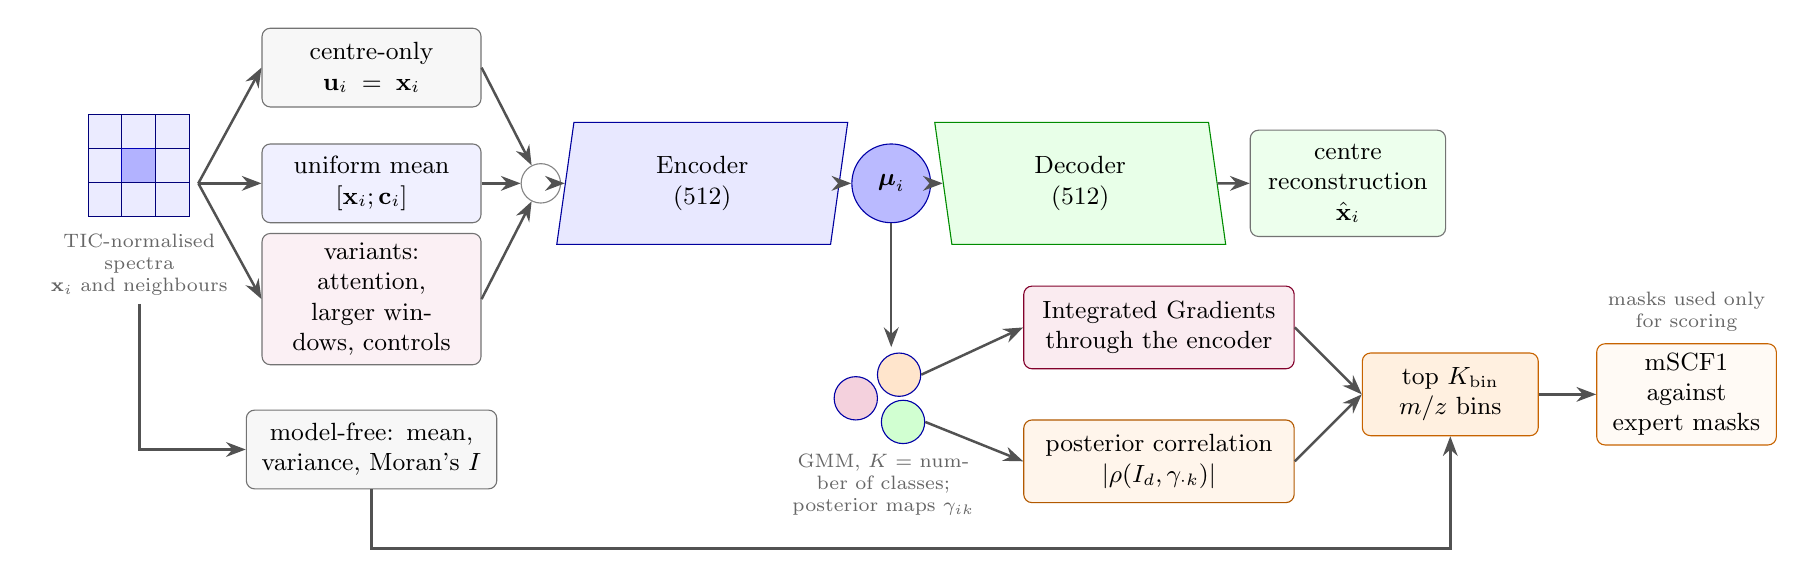
\begin{tikzpicture}[font=\sffamily]
  % Section grid (input spectra).
  \foreach \r in {0,1,2}{\foreach \c in {0,1,2}{
    \pgfmathtruncatemacro{\iscenter}{(\r==1 && \c==1)}
    \ifnum\iscenter=1
      \filldraw[draw=blue!72!black, fill=blue!30] ($(0.0,0.65)+(0.43*\c,-0.43*\r)$) rectangle ++(0.43,-0.43);
    \else
      \filldraw[draw=blue!48!black, fill=blue!8] ($(0.0,0.65)+(0.43*\c,-0.43*\r)$) rectangle ++(0.43,-0.43);
    \fi}}
  \node[label, text width=2.6cm] at (0.65,-1.25) {TIC-normalised spectra\\$\mathbf{x}_i$ and neighbours};

  % Encoder input options.
  \node[block, fill=black!3, text width=2.5cm, minimum height=1.0cm] (central) at (3.6,1.25) {centre-only\\$\mathbf{u}_i=\mathbf{x}_i$};
  \node[block, fill=blue!6, text width=2.5cm, minimum height=1.0cm] (uniform) at (3.6,-0.22) {uniform mean\\$[\mathbf{x}_i;\mathbf{c}_i]$};
  \node[block, fill=purple!6, text width=2.5cm, minimum height=1.0cm] (attention) at (3.6,-1.69) {variants: attention,\\larger windows, controls};
  \node[circle, draw=black!48, fill=white, minimum size=0.5cm, inner sep=0pt] (merge) at (5.75,-0.22) {};
  \node[encoder] (enc) at (7.8,-0.22) {Encoder\\(512)};
  \node[latent, fill=blue!27, minimum size=1.0cm] (z) at (10.2,-0.22) {$\boldsymbol{\mu}_i$};
  \node[decoder] (dec) at (12.6,-0.22) {Decoder\\(512)};
  \node[block, fill=green!7, text width=2.2cm] (recon) at (16.0,-0.22) {centre\\reconstruction $\hat{\mathbf{x}}_i$};
  \foreach \n in {central,uniform,attention}{\draw[flow] (1.4,-0.22) -- (\n.west); \draw[flow] (\n.east) -- (merge);}
  \draw[flow] (merge.east) -- (enc.west);
  \draw[flow] (enc.east) -- (z.west);
  \draw[flow] (z.east) -- (dec.west);
  \draw[flow] (dec.east) -- (recon.west);

  % GMM segmentation.
  \node[latent, minimum size=0.55cm, fill=purple!18] (g1) at (9.75,-2.95) {};
  \node[latent, minimum size=0.55cm, fill=orange!20] (g2) at (10.3,-2.65) {};
  \node[latent, minimum size=0.55cm, fill=green!18] (g3) at (10.35,-3.25) {};
  \node[label, text width=3.4cm] at (10.1,-4.05) {GMM, $K$ = number of classes;\\posterior maps $\gamma_{ik}$};
  \draw[flow] (z.south) -- (10.2,-2.3);

  % Two ranking branches from the same GMM.
  \node[peakbox, text width=3.2cm] (ig) at (13.6,-2.05) {Integrated Gradients\\through the encoder};
  \node[peakbox, fill=orange!8, draw=orange!70!black, text width=3.2cm] (pcc) at (13.6,-3.75) {posterior correlation\\$|\rho(I_d,\gamma_{\cdot k})|$};
  \draw[flow] (g2.east) -- (ig.west);
  \draw[flow] (g3.east) -- (pcc.west);

  % Model-free rankings from the spectra.
  \node[block, fill=black!3, text width=2.9cm, minimum height=1.0cm] (free) at (3.6,-3.6) {model-free: mean,\\variance, Moran's $I$};
  \draw[flow] (0.65,-1.75) |- (free.west);

  % Output and evaluation.
  \node[outbox, text width=2.0cm] (peaks) at (17.3,-2.9) {top $K_{\text{bin}}$\\$m/z$ bins};
  \draw[flow] (ig.east) -- (peaks.west);
  \draw[flow] (pcc.east) -- (peaks.west);
  \draw[flow] (free.south) -- ++(0,-0.75) -| (peaks.south);
  \node[block, fill=orange!4, draw=orange!78!black, text width=2.0cm, minimum height=0.95cm] (score) at (20.3,-2.9) {mSCF1 against\\expert masks};
  \draw[flow] (peaks.east) -- (score.west);
  \node[label, text width=2.4cm] at (20.3,-1.85) {masks used only\\for scoring};
\end{tikzpicture}
\end{document}
